\documentclass[12pt, oneside]{article}
\usepackage{geometry}                		% See geometry.pdf to learn the layout options. There are lots.
\geometry{letterpaper} 
\usepackage{amsmath}
\usepackage{amsthm}
\usepackage{amssymb}
\usepackage{graphicx}
\usepackage{color}
\usepackage{float}
\usepackage{subfig}
\usepackage[flushleft]{threeparttable}
\usepackage{gensymb}
\usepackage{multirow}
\usepackage[dvipsnames]{xcolor}
\newcommand{\BibTeX}{\textsc{Bib}\TeX}
%opening
\title{Using CutGridFlow}
\author{}

\begin{document}



\section{Setting up the new domain}


\begin{figure}[H]
\centering
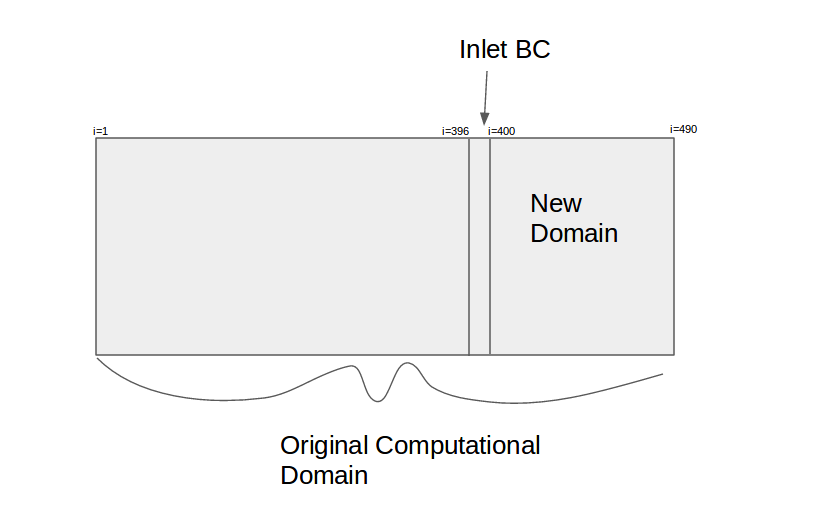
\includegraphics[width=0.5\textwidth]{FIGS/GridCut.png}

\caption{{\footnotesize Grid Cut}}
\label{fig: } 
\end{figure}

\subsection{Making the inlet file }

\begin{figure}[H]
\centering
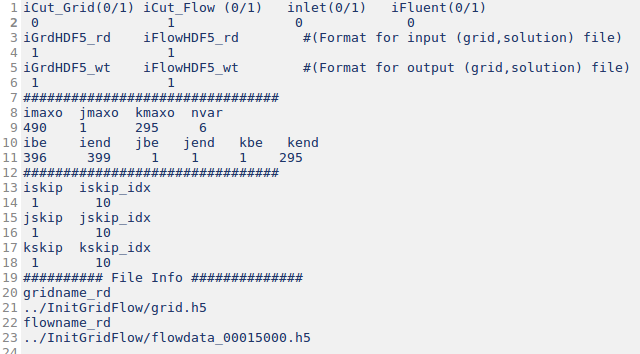
\includegraphics[width=0.5\textwidth]{FIGS/ExampleInlet.png}

\caption{Example Input File for making inlet}
\label{fig: } 
\end{figure}

iCut\_Grid should be set to 0, while iCut\_flow should be set to 1. \newline
The rd and wt tags should be set to values based on your input file types and desired output file type. \newline
The maxo variables should be the last index of each direction of your input file \newline
ibe and iend should be set to the 4 indexes before the desired zone for the new computational domain \newline
The File Info section should contain the file location for your input files, it is \newline recommended that they be located in a different location otherwise the files will be overwritten. \newline
The CutGridFlow program should then be run and the output, flowdata\_00000000.h5, file should be renamed to inlet.h5

\subsection{Making the inletgrid file }

\begin{figure}[H]
\centering
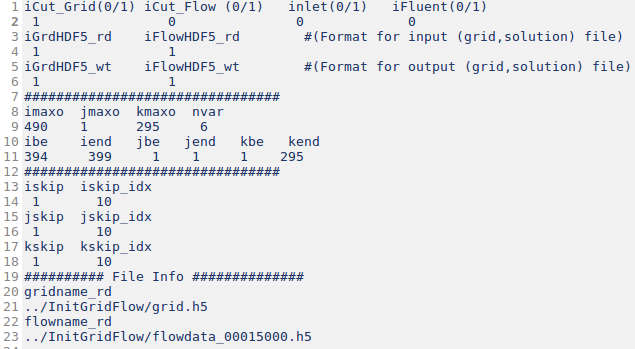
\includegraphics[width=0.5\textwidth]{FIGS/ExampleInletgrid.png}

\caption{{\footnotesize Example Input File for making inletgrid}}
\label{fig: } 
\end{figure}

iCut\_Grid should be set to 1, while iCut\_flow should be set to 0 now. \newline
ibe and iend should be set to the 6 indexes before the desired zone for the new computational domain. This will mean ibe is 2 less than when making the inlet file. \newline
The CutGridFlow program should then be run and the output, grid.h5, file should be renamed to inletgrid.h5



\subsection{Making the new Flowdata and Grid files}

\begin{figure}[H]
\centering
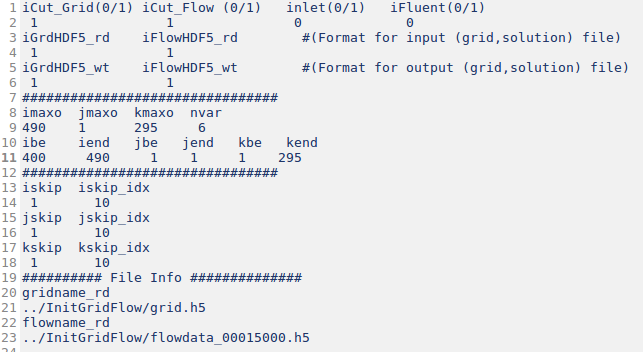
\includegraphics[width=0.5\textwidth]{FIGS/ExampleInputND.png}

\caption{{\footnotesize Example Input File for making new computational domain}}
\label{fig: } 
\end{figure}

Both iCut tags should be set to 1 now. \newline
The ibe and iend should be set to the area from the input files to be used for the new computational domain. \newline
The program should now be run, if you are not using a flowdata\_00000000.h5 file for input you will need to rename the output to match your input afterwards.

\section{Using the new domain}

Setting up the DNS code will be the same as for other cases with the exception of one of the boundary conditions. The inletbc should be set to 1 and the inletdatatype should be set to 2. 
This will require that the inlet and inletgrid files will need to be accessible from the same folder as the deck3d.inp file. \newline
Remember to change RunParams as needed, reindex the sponge zones and turn off the inlet sponge







\end{document}